La placa de XIAO ESP32S3 es el elemento fundamental de la parte frontal del contenedor. El corazón del sistema. Se encarga de reconocer el desecho solido a ser depositado, para ello se utilizan componentes que dotan a la placa de mayores capacidades. Destacan tres:

\begin{itemize}
  \item \textbf{Sensor de cámara OV2640:} viene includo en una placa de expansión de cámara, la cual se conecta a la ESP32S3 mediante un módulo de cámara integrado que trae de fábrica la placa.
  \item \textbf{Puerto MicroSD:} al igual que el  módulo de cámara viene incluido en la placa de expansión de cámara. Este puerto permite, entre otras cosas, guardar las imágenes tomadas por la cámara. Esto con el fin de entrenar la red neuronal convolucional.
  \item \textbf{Antena de comunicación WiFi/Bluetooth:} esta antena permite enviar información de la placa al teléfono. Esto se usa para informar sobre el nivel de llenado del contenedor.
\end{itemize}

En primer lugar hay que conseguir las imagenes para entrenar el modelo. Para ello se hace uso de un código mediante el cual se le transfiere a la ESP32S3, con el sensor de cámara acoplado para poder capturar las imágenes, la opción de guardar imágenes. Estas imágenes se almecenan una tarjeta MicroSD. En una computadora se suben las imágenes en la MicroSD a la plata forma \emph{Edge Impulse} para proceder a entrenar el modelo.

A la placa se le carga un modelo de red neuronal convolucional (CNN) que está entrenada para reconocer dos tipos de objetos: cartón y plástico. La detección de estos objetos está condicionada en gran medida por como fue entrenada la red, dado que circunstancias como el ángulo de la imagen y/o la cámara, iluminación, calidad de imágen y otros pueden afectar el resultado.

\begin{figure}[htb]
	\centering
	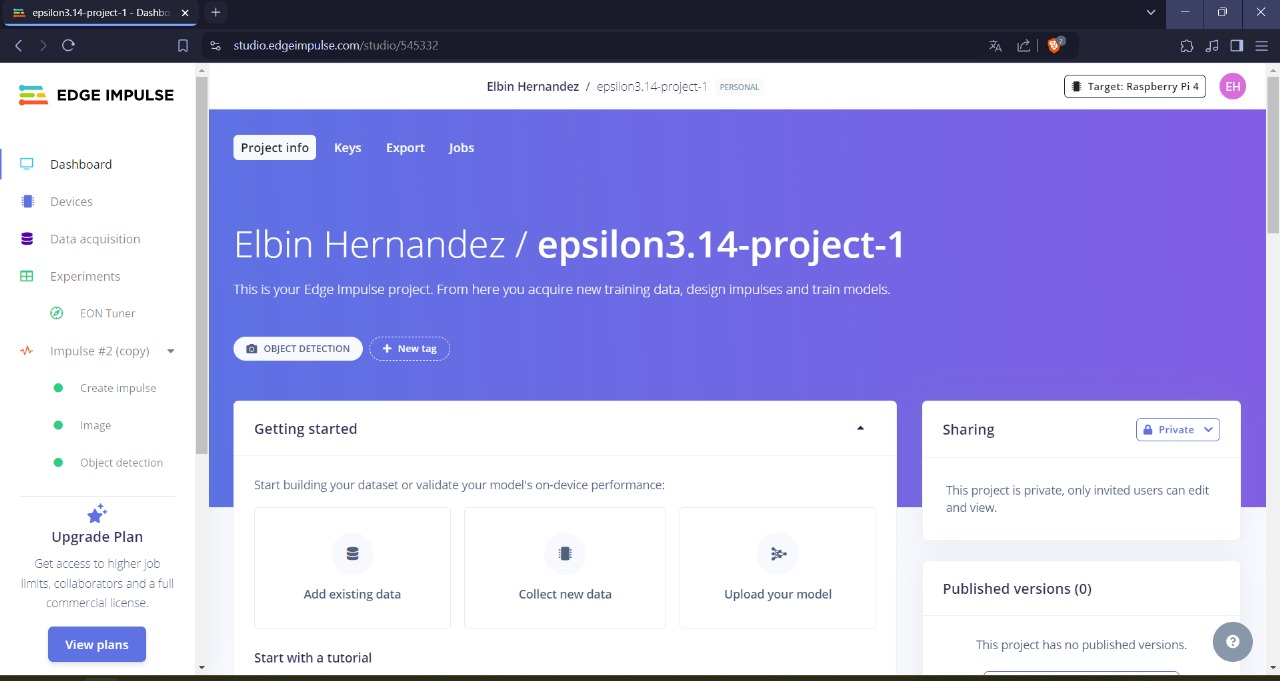
\includegraphics[scale  = 0.4]{Imagenes/plataforma_edge.jpeg}
	\caption{Plataforma Edge Impulse}{Fuente: Propia}
\end{figure}

\begin{figure}[H]
	\centering
	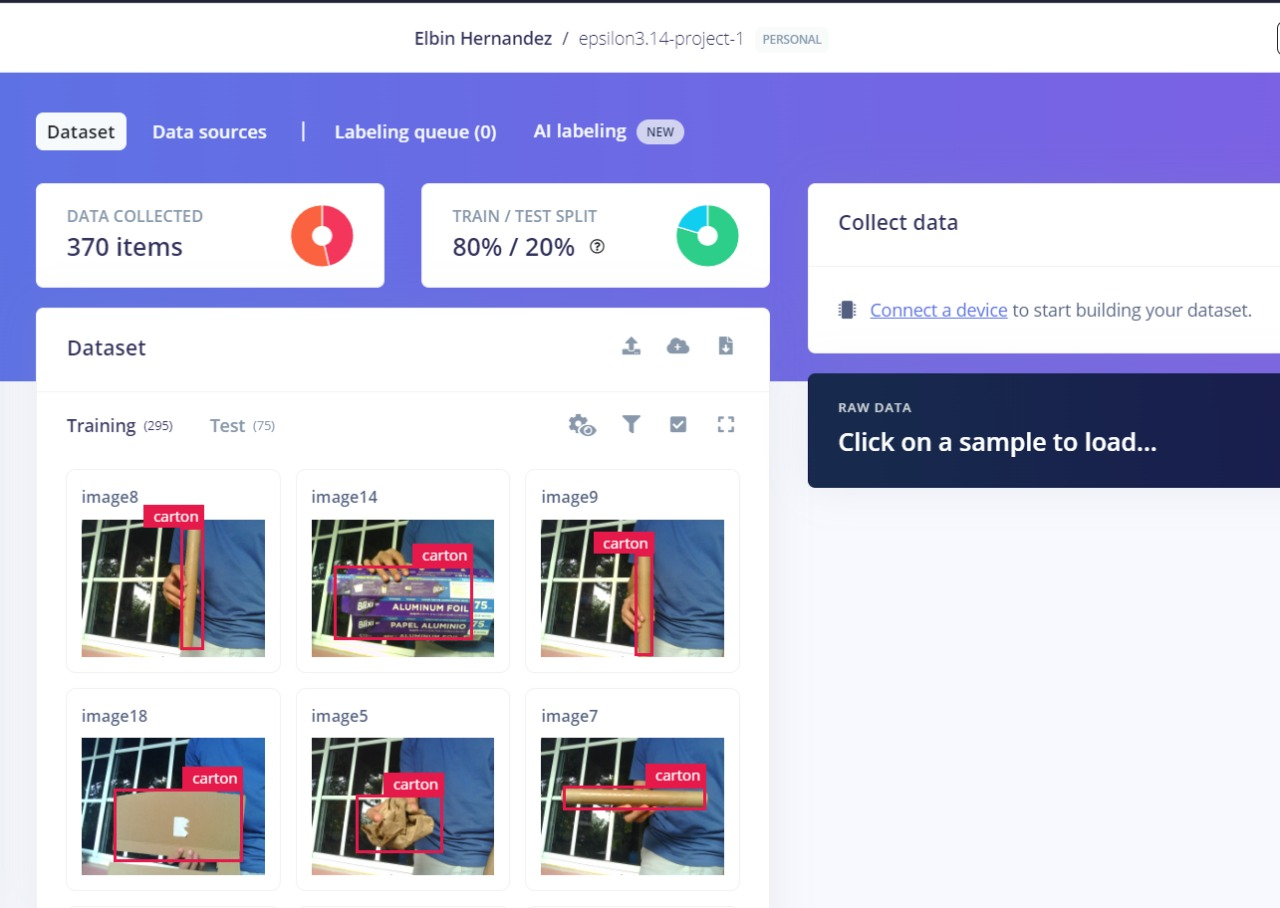
\includegraphics[scale  = 0.4]{Imagenes/datos_plataforma.jpeg}
	\caption{Datos plataforma Edge Impulse}{Fuente: Propia}
\end{figure}

La red neuronal es entrenada en la plataforma \emph{Edge Impulse} utilizando imágenes tomadas con el sensor de cámara OV2640. Estas imágenes fueron subidas a la plataforma y haciendo uso de las herramientas que provee se entrenó la red. Hay dos tipo de imágenes: \emph{training} y \emph{testing}. Las primeras se utilizaron para que la red aprendiese a reconocer cartón y plástico. Mientras que las segundas para poner a prueba la efectividad de la red con imágenes con las nunca había interactuado. Las imágenes fueron etiquetadas como cartón y plástico.

\begin{figure}[htb]
	\centering
	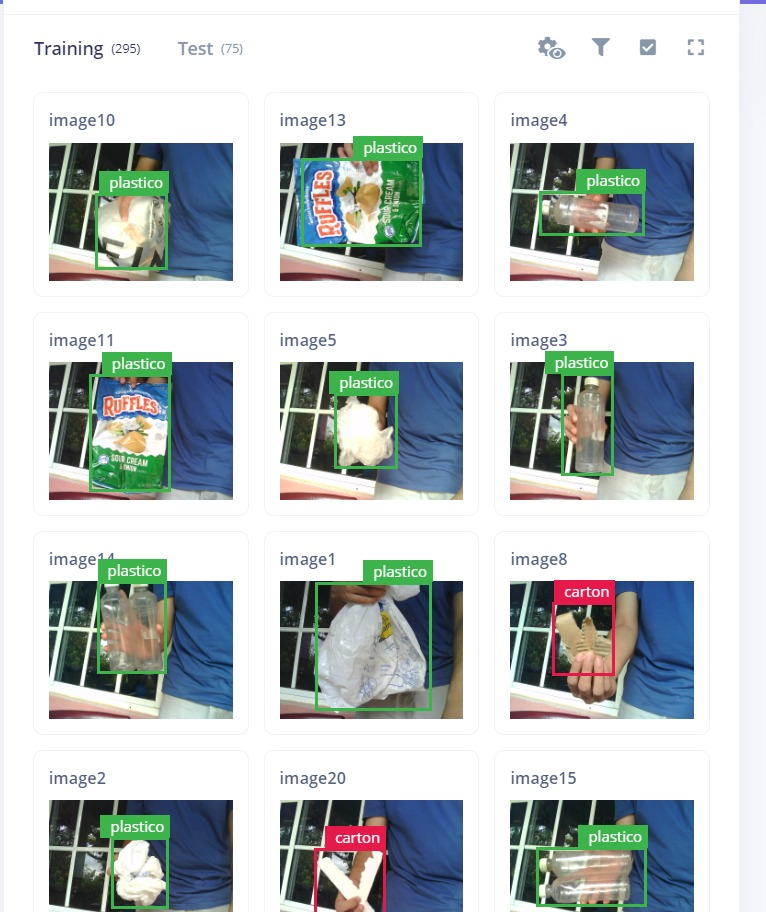
\includegraphics[scale  = 0.4]{Imagenes/imagenes_training.jpeg}
	\caption{Imágenes de entrenamiento}{Fuente: Propia}
\end{figure}

\begin{figure}[H]
	\centering
	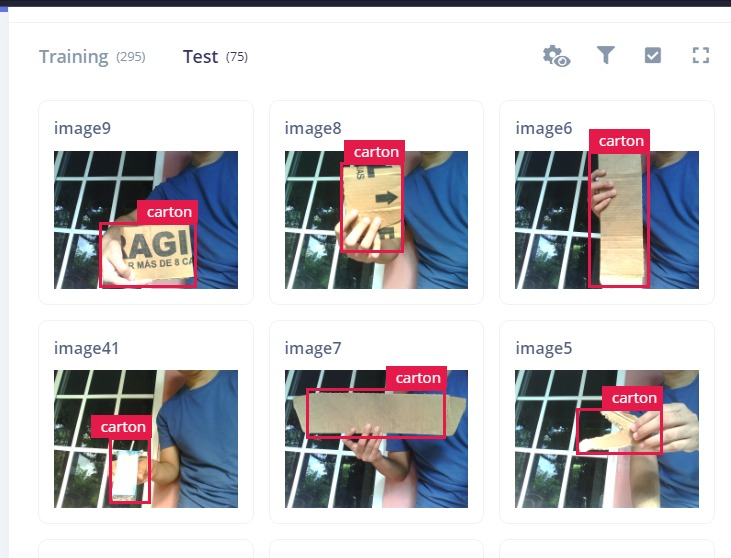
\includegraphics[scale  = 0.4]{Imagenes/imagenes_testing.jpeg}
	\caption{Imágenes de prueba}{Fuente: Propia}
\end{figure}

\begin{figure}[htb]
	\centering
	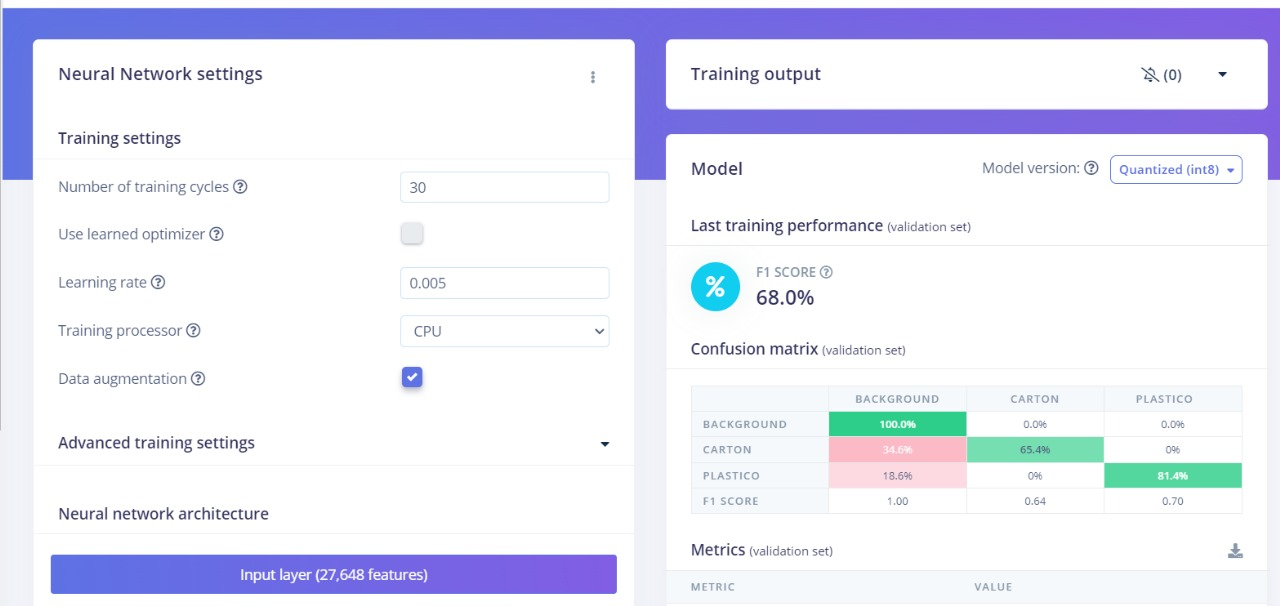
\includegraphics[scale  = 0.4]{Imagenes/stat_modelo.jpeg}
	\caption{Estadísticas de la red neuronal}{Fuente: Propia}
\end{figure}

\begin{figure}[H]
	\centering
	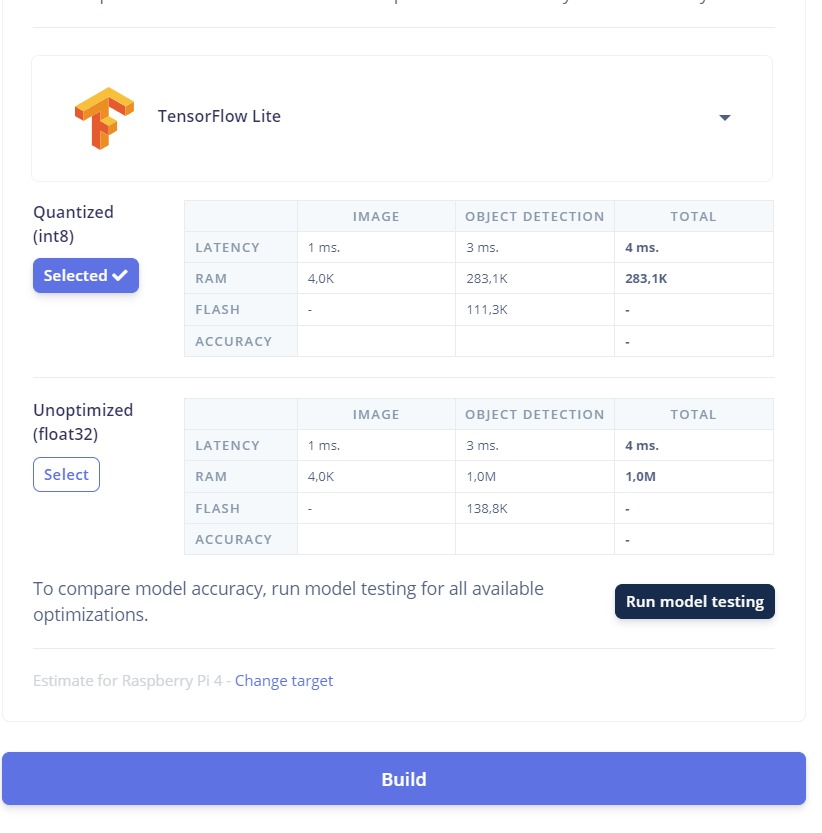
\includegraphics[scale  = 0.4]{Imagenes/modelo_tensor.jpeg}
	\caption{Modelo TensorFlow Lite}{Fuente: Propia}
\end{figure}

Tras detectar un objeto envia la etiqueta, en forma de texto mediante la consola serial en el puerto \emph{115200}, que identifica a ese objeto al Arduino Uno, para que este evalue que servomotor debe activarse para abrir la compuerta correspondiente. De manera paralela y constante, establece un proxy mediante la antena de comunicación inalámbrica que contiene la información del porcentaje de llenado del contenedor. Esta señal puede ser captada por un teléfono y mediante una aplicación se puede visualizar y monitorear constantemente el nivel de desechos en el contenedor. 

La ESP32S3 envia la información mediante el pin digital 6, el cual funciona como el pin TX y mediante un cable se conecta al pin 1 de arduino, que corresponde al RX. Por tanto, realizando esta conexión se establece un comunicación rápida entre ambas placas.

\begin{figure}[H]
	\centering
	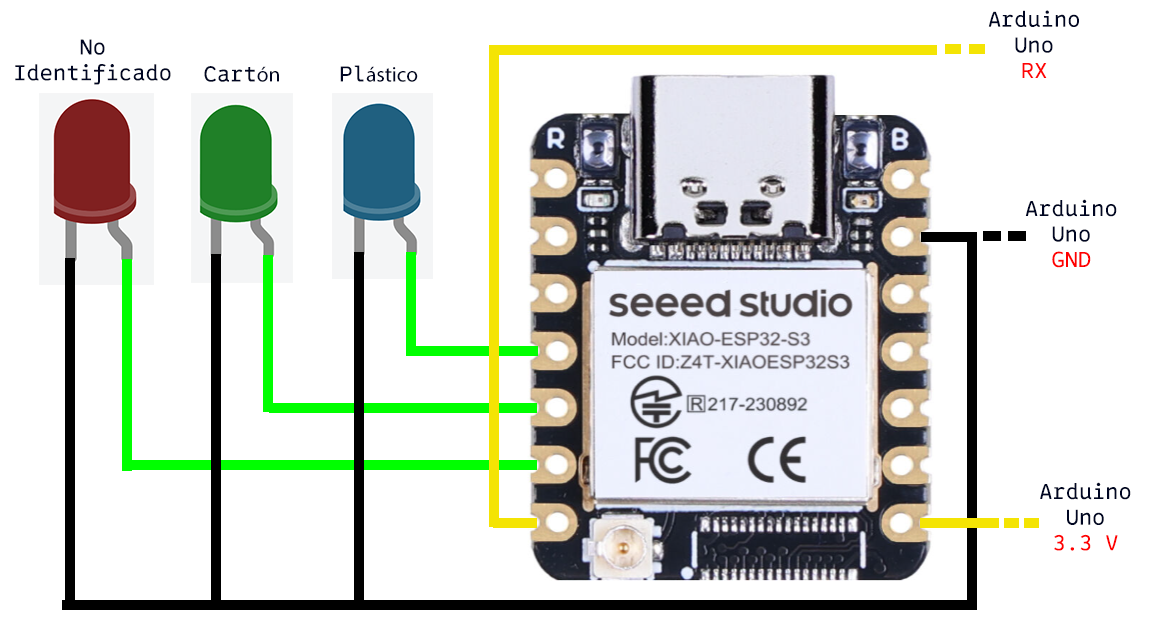
\includegraphics[scale  = 0.50]{Imagenes/esp32s3_coneccion.png}
	\caption{Conexión de la placa ESP32S3}{Fuente: Propia}
\end{figure}

A continuación se presenta el código de la placa ESP32S3:

\lstinputlisting[style = arduinostyle]{Codigos/codigo_esp32s3.ino}